%!TEX TS-program = xelatex
%!TEX encoding = UTF-8

% Unit pembaca Bahasa Indonesia untuk Methods of Algebra, Volume 1.
% Teks sumber: Copyright 2018 Wen-Wei Li, CC BY 4.0.
% Terjemahan ini dilisensikan menurut CC BY 4.0.

\documentclass[
	colors = true,
	coverpage = coverpage-id-unit-001.tex,
	fontsetup = font-setup-id.tex,
	titlesetup = titles-setup.tex,
	CJKthechapter = false
]{AJbook}

\newcommand{\BuildDateID}{21 Agustus 2026}
\newcommand{\BuildDateShortID}{2026-08-21}

\usepackage{mathrsfs}
\usepackage{stmaryrd}
\SetSymbolFont{stmry}{bold}{U}{stmry}{m}{n}
\usepackage{array}
\usepackage{makecell}
\usepackage{tabularx}
\newcolumntype{Y}{>{\raggedright\arraybackslash}X}
\usepackage{tikz-cd}
\usetikzlibrary{positioning, patterns, calc, matrix, shapes.arrows, shapes.symbols}
\usepackage{braids}
\usepackage{tqft}
\usepackage{ytableau}
\usepackage{pgfplots}
\pgfplotsset{compat=1.18}
\usepackage{myarrows}
\usepackage{mycommand}

\usepackage[noautomatic]{imakeidx}
\makeindex[
	columns=2,
	program=makeindex,
	intoc=true,
	title={Indeks Istilah}]

\usepackage{xr}
\usepackage[unicode, bookmarksnumbered]{hyperref}
% Import only the frozen numbers.  The empty URL deliberately prevents the
% standalone unit from creating links to a PDF that is not shipped with it.
\externaldocument{unit-001-crossrefs}[]
\hypersetup{
	pdfauthor = {Wen-Wei Li},
	pdftitle = {Metode Aljabar, Jilid 1: Arsitektur Dasar - Unit 1: Pendahuluan},
	pdfsubject = {Terjemahan Bahasa Indonesia independen},
	pdfkeywords = {aljabar, kategori, struktur aljabar, id-ID},
	pdflang = {id-ID},
	CJKbookmarks = true}

\addbibresource{Al-jabr.bib}

\begin{document}
	% Cover and contents pages deliberately have no page anchors.  This avoids
	% collisions when \mainmatter restarts Arabic numbering at page 1.
	\hypersetup{pageanchor=false}
	\pagestyle{empty}
	\input{coverpage-id-unit-001.tex}
	\pagestyle{fancy}
	\pagenumbering{roman}
	\setcounter{page}{1}
	\renewcommand{\contentsname}{Daftar Isi}
	\tableofcontents

	\mainmatter
	\hypersetup{pageanchor=true}
	% Sumber LaTeX terjemahan bahasa Indonesia dari buku ``代数学方法'' (Metode Aljabar).
% Copyright 2018  李文威 (Wen-Wei Li).
% Permission is granted to copy, distribute and/or modify this
% document under the terms of the Creative Commons
% Attribution 4.0 International (CC BY 4.0)
% http://creativecommons.org/licenses/by/4.0/

% To be included
\chapter*{Pendahuluan}	% Kelas dokumen otomatis menambahkannya ke daftar isi dan mengatur kepala halaman.

\section*{Gambaran umum}
Istilah aljabar berasal dari karya cendekiawan Persia abad ke-9, al-Khwārizmī. Ketika Li Shanlan dan A.\ Wylie menerjemahkan \textit{Elements of Algebra} karya A.\ De Morgan bersama-sama pada tahun 1859, mereka menjelaskannya sebagai seni ``melengkapi dan meniadakan'', yakni keterampilan menyelesaikan persamaan, yang kurang lebih setara dengan matematika sekolah menengah dewasa ini. Sejak abad ke-20, cakupan aljabar meluas hingga mencakup objek matematika dan operasinya secara lebih umum. Peralihan ini bermula dari serangkaian karya E.\ Noether dan tokoh-tokoh lain, lalu memperoleh bentuk awalnya dalam karya besar B.\ L.\ van der Waerden, \textit{Algebra}\cite{vdW1, vdW2}. Dalam pengertian ini, objek-objek dasar aljabar secara kasar dapat dibagi menjadi grup, gelanggang, modul, dan medan. Dengan kosakata mazhab Bourbaki, matematika dapat dipandang sebagai jalinan rumit berbagai struktur beserta transformasi di antaranya; suatu struktur aljabar adalah himpunan yang dilengkapi operasi tertentu, misalnya bilangan rasional dengan empat operasi aritmetika membentuk medan bilangan rasional $\Q$. Secara ringkas, aljabar adalah kajian mengenai struktur aljabar.

Dimulai dengan tinjauan seperlunya atas teori himpunan, buku ini memakai sudut pandang teori kategori untuk menjalin pembahasan grup, gelanggang, modul, medan, dan berbagai konsep turunannya. Keseluruhan inilah yang membentuk ``arsitektur dasar'' dalam subjudul buku ini.

Dalam susunan perkuliahan yang lazim saat ini, mata kuliah aljabar biasanya ditempuh setelah analisis matematika serta aljabar lanjut, yakni aljabar linear. Sebagai contoh, di University of Chinese Academy of Sciences (UCAS), tempat penulis pernah mengajar, mahasiswa berkenalan dengan kosakata teori himpunan dan topologi himpunan titik dalam mata kuliah kalkulus. Mata kuliah aljabar linear membekali mereka dengan teori dasar ruang vektor dan polinom, sekaligus contoh-contoh awal grup, gelanggang, dan medan. Dengan dasar ini, struktur aljabar yang lebih umum dapat dipelajari dengan mudah, dan teori Galois bagi perluasan hingga menjadi ujian puncaknya. Susunan pengajaran berbeda-beda antarlembaga, tetapi pentingnya kematangan aljabar diakui oleh semua matematikawan. Hal ini bukan sekadar untuk memupuk kepekaan estetis: di mana pun struktur aljabar muncul, di sana metode aljabar dapat digunakan. Daftar nama bidang yang terkait—teori bilangan aljabar, geometri aljabar, topologi aljabar, kombinatorika aljabar, bahkan statistika aljabar—sudah memberi gambaran kasar tentang kegunaan keterampilan ini. Penerapan metode aljabar dalam fisika, kimia, ilmu komputer, dan bidang-bidang lain pun dikenal luas.

Pokok bahasan buku ini kadang disebut pula ``aljabar modern'' atau ``aljabar abstrak''. Sebutan modern selalu relatif terhadap zamannya; ketika menerbitkan edisi keempat \textit{Algebra} pada tahun 1955, van der Waerden sudah meninggalkan kata itu, sehingga kini semakin tidak diperlukan. Adapun sebutan abstrak, paling jauh ia hanya mencerminkan kesan keliru seorang pemula. Sebagai nama mata kuliah atau buku, sebutan itu sama sekali tidak mengenai pokok persoalan dan malah terkesan menggentarkan pembaca. Buku ini diberi judul ``Metode Aljabar'', pertama karena cakupan aljabar masa kini terlalu luas: buku ini hanya memilih hal-hal yang menarik dan berguna, tanpa berusaha membangun sistem yang serba lengkap. Alasan kedua, dan yang terpenting, ialah bahwa hakikat matematika terletak pada pertautan dan saling pengaruh antarbagiannya; pengelompokan di bawah satu istilah dibuat hanya demi kemudahan pengajaran dan pembagian disiplin. Karena itu, buku ini sama sekali tidak memandang aljabar sebagai bidang dengan batas tegas. Seandainya aljabar murni yang terpisah dari analisis, topologi, dan bidang lain memang ada, ia hanyalah salah satu dari tak terhitung banyaknya arah penelitian. Dalam bab ``Ying Di Wang'' dari Zhuangzi terdapat kisah tentang tujuh lubang yang dipahatkan pada Hundun; memaksakan batas-batas pun dapat membuat matematika mandek dan mati.

Isi banyak buku ajar aljabar sarjana kira-kira berhenti pada keadaan tahun 1950-an hingga 1960-an. Ini sama sekali tidak berarti bahwa isi dan metode aljabar telah mencapai bentuk akhirnya. Justru sebaliknya, sejak itu matematika mengalami perkembangan yang belum pernah terjadi sebelumnya, termasuk lahirnya pemahaman baru yang lebih mendalam atas tema-tema klasik. Dalam cakupan buku ini, kebangkitan teori kategori kiranya merupakan perkembangan yang paling menonjol. Berkat topologi, teori ini membangun suatu filsafat hubungan dalam matematika: yang sungguh penting bukanlah ``apa'' suatu struktur matematika itu—misalnya, unsur apa saja yang dimilikinya sebagai himpunan—melainkan hubungan antarstruktur, atau fungsi dan peran struktur tersebut. Penulis secara khusus ingin menekankan sumbangan topologi, terutama teori homotopi. Hingga kini aljabar terus memperoleh perkakas dan tantangan baru darinya. Asal-usul ini tidak sulit dipahami melalui intuisi topologis; melewatkannya begitu saja karena sekat disiplin yang direka-reka akan sangat merugikan pembaca.

Tentu saja, teori yang benar-benar agung mampu melampaui zamannya dan terus memancarkan cahaya. Bagaimana kita dapat menangkap sarinya dalam bentuk modern, memangkas cabang-cabang yang tidak perlu tanpa mengurangi kecemerlangan aslinya? Itulah tujuan yang ditetapkan penulis bagi dirinya. Jelas tidak realistis untuk mencapainya sekaligus; karena itu, beberapa tema dalam buku ini akan diperlakukan dari sudut pandang klasik atau ``semiklasik''.

Perlu pula dijelaskan bahwa urutan sejarah berbeda dari urutan konsep. Pada umumnya, konsep baru jarang beroleh pijakan dalam matematika karena sejak awal sederhana dan tembus pandang. Justru sebaliknya: konsep itu harus lebih dahulu membuktikan daya gunanya pada masalah lama yang paling sulit. Walaupun konsep baru pada akhirnya menjadi batu penjuru bangunan masa depan, masalah lama justru berubah menjadi latihan bagi mahasiswa. Akibatnya, kerangka teori tampak sebagai hal utama, sedangkan penerapan tampak sebagai sesuatu yang datang dari luar dan bersifat turunan. Kita harus mengakui bahwa rekonstruksi semacam ini merupakan jalan yang tak terelakkan dalam belajar, sekaligus salah satu tanda kemajuan matematika. Namun, pembaca juga perlu memahami bahwa berbagai konsep aljabar tidak hanya mendirikan bangunan-bangunan yang kukuh; jika dilihat dari silsilahnya, konsep-konsep itu lebih menyerupai jaring besar dengan simpul-simpul yang saling menopang. Pada tataran metode, hal ini menuntut pelajar untuk bergerak luwes dan melihat hubungan ke segala arah.

Persiapan awal buku ini dapat ditelusuri hingga sekitar tahun 2013. Dalam pergaulan dengan mahasiswa dari berbagai tempat, penulis sangat terkesan oleh bakat dan semangat mereka. Di pihak lain, dukungan yang mampu atau bersedia diberikan oleh sekolah dan para pengajar sangat tidak sebanding dengan bakat dan semangat itu. Sayangnya, internet belum juga mengatasi ketimpangan sumber daya ini. Bahkan jika seorang yang berwawasan luas merekomendasikan sebuah buku ajar, isinya umumnya sudah ketinggalan zaman; begitu pembaca memasuki ranah penelitian, hambatan pun segera tampak. Berdasarkan pertimbangan ini, penyusunan buku menetapkan beberapa sasaran:
\begin{itemize}
	\item berfungsi sekaligus sebagai bahan belajar mandiri, buku rujukan, dan sumber pengajaran;
	\item mengacu pada kebutuhan penelitian nyata, terutama pembaruan gagasan dan notasi;
	\item menonjolkan keterbukaan dan menekankan pertautan aljabar dengan berbagai masalah lain.
\end{itemize}
Karena itu, buku ini bukan buku ajar yang dirancang khusus untuk satu mata kuliah atau satu lembaga. Bab-babnya tidak harus sejalan dengan urutan pengajaran ataupun jumlah jam kuliah. Baik pengajar maupun pembelajar mandiri hendaknya memilih materi sesuai kebutuhan mereka sendiri.

Walaupun struktur sebuah buku ajar harus berkembang secara linear, dalam pembelajaran nyata berbagai tema niscaya bersilangan dan berulang, seperti sebilah pedang yang ditempa berulang kali; inilah hukum alamiah dalam menyerap pengetahuan baru. Namun, kelompok yang berbeda memerlukan irama belajar yang berbeda, apalagi jika buku digunakan sebagai rujukan. Jalan tengah yang ditempuh buku ini adalah memakai urutan logis sebagai jangkar secara garis besar, sedangkan lompatan dan tinjauan balik yang diperlukan diwujudkan melalui rujukan silang. Bagi pembaca yang telah memiliki dasar aljabar tertentu, setiap bab kurang lebih dapat dibaca secara mandiri apabila rujukan silang dan indeks di akhir buku dimanfaatkan dengan baik.

Sebagian isi buku ini pernah diajarkan dalam mata kuliah sarjana dan pascasarjana di University of Chinese Academy of Sciences (UCAS). Dalam proses penulisannya, buku ini merujuk secara luas pada buku ajar yang telah ada, termasuk tetapi tidak terbatas pada Bourbaki \cite{Bou-Alg1, Bou-Alg2}, Jacobson \cite{Ja85, Ja89}, Lang \cite{Lang02}, MacLane \cite{ML98}, van der Waerden \cite{vdW1,vdW2}, dan lain-lain. Sumber daring seperti \href{http://mathoverflow.net}{MathOverflow} dan \href{http://ncatlab.org}{nLab} juga dimanfaatkan. Buku ajar berbahasa Tionghoa karya Zhang Herui \cite{ZHR} dan Nie Lingzhao--Ding Shisun \cite{DN00} pun memberikan banyak bahan pembanding. Penulis menyampaikan penghormatan kepada semuanya dari kejauhan. Karena keterbatasan pengetahuan dan tenaga, kesalahan atau kekurangan tentu sulit dihindari; penulis sangat mengharapkan koreksi dari para ahli.

Selama penyusunan buku ini, penulis menerima pengertian dan bantuan dari banyak guru, sahabat, dan mahasiswa. Sejauh yang dapat diingat, nama-nama berikut dicantumkan sebagai ungkapan terima kasih: Bai Chenyu, Feng Qi, Li Jinghui, Liu Xin, Mao Shengkai, Ming Yang, Rong Shi, Shan Ning, Tao Jinghui, Wang Dan, Xi Nanhua, Xiong Rui, Zhang Bingyu, Zhang Hao, Zhou Shengxuan, Zhu Renjie, dan Zou Changhan {\small(diurutkan menurut pinyin)}. Selain itu, editor Zhao Tianfu dari Higher Education Press memberikan banyak saran profesional; kepadanya penulis juga menyampaikan terima kasih.\nopagebreak

\vspace{1em}
\begin{flushright}\begin{minipage}{0.58\textwidth}
	\begin{tabular}{c}
		{\kaishu Wen-Wei Li} \\
		Maret 2018, di sebelah selatan Jembatan Baofusi
	\end{tabular}
\end{minipage}\end{flushright}
\vspace{1em}

\section*{Prasyarat}
Buku ini tidak berusaha membangun suatu sistem yang mandiri atau berbatas tegas. Lagi pula, pengalaman umum dalam penelitian menunjukkan bahwa jika seseorang menunggu hingga segala sesuatu siap sebelum berani membuka wilayah baru, biasanya tidak ada apa pun yang tercapai; hal ini terutama berlaku pada bidang-bidang yang berkaitan dengan aljabar. Dalam membaca, kita tak terhindarkan akan menjumpai pokok pengetahuan yang baru atau belum dikuasai dengan kukuh. Sikap yang lebih tepat barangkali ialah ``menarik implikasinya dan memperluas pemahaman melalui hal-hal yang sejenis''. Meskipun demikian, tetap perlu digambarkan suatu ambang minimum yang samar. Menurut perkiraan konservatif, buku ini mengharapkan pembaca telah menguasai dengan baik mata kuliah tahun-tahun awal program studi matematika di perguruan tinggi. Jika pembaca juga pernah mengikuti satu semester mata kuliah aljabar tingkat sarjana, misalnya paruh pertama \cite{DN00} atau \cite{ZHR}, sebagian besar isi buku ini semestinya dapat dipahami dengan lancar, tetapi hal itu bukan keharusan. Keadaan khusus tentu perlu dinilai secara khusus, bergantung pada pengalaman belajar dan berpikir masing-masing pembaca serta keberaniannya.

Berikut beberapa kelompok prasyarat yang terkait, disusun menurut bobotnya dari yang terbesar ke yang terkecil.
\begin{description}
	\item[Kematangan dasar] Ini mencakup bahasa logika, metode pembuktian seperti kontradiksi dan rekursi, pengetahuan umum tentang himpunan dan kefasihan menggunakan simbol, pemahaman awal tentang struktur matematika, kepekaan terhadap bahasa abstrak, dan sebagainya—singkatnya, ``kematangan''. Aspek dasarnya tercakup dalam pelajaran sekolah menengah atau tahun pertama perguruan tinggi; pada taraf yang mendalam, hal ini merupakan pekerjaan seumur hidup seorang matematikawan.
	\item[Matriks, ruang vektor, polinom] Di Tiongkok, materi ini umumnya tercakup dalam mata kuliah aljabar lanjut atau aljabar linear tahun pertama, misalnya \cite{Xi16, Xi18}, sedangkan bagian elementernya juga diajarkan di sekolah menengah. Pembaca hendaknya memiliki pemahaman paling dasar tentang matriks dan ruang vektor, serta mengetahui hubungan antara matriks dan transformasi linear; pengetahuan tentang cara kerja permutasi (grup simetris) akan lebih baik lagi. Walaupun semua tema ini dapat digolongkan ke dalam aljabar, latar belakang kebanyakan pembaca maupun kemudahan penyajian tidak menuntut agar semuanya dijelaskan dari awal. Dalam buku ini, pengetahuan tersebut terutama dipakai untuk memberi contoh dan mempersingkat pembuktian; pilihan untuk menggunakannya tidak memengaruhi batang utama teori.
	\item[Teori bilangan elementer] Ini meliputi pengetahuan umum tentang keterbagian, faktorisasi prima, algoritma Euklides, serta perluasannya pada polinom. Selain itu, pembaca hendaknya mengenal, atau setidaknya bersedia menerima, penggunaan kongruensi, terutama modulo bilangan prima $p$. Hasil paling dasar seperti teorema kecil Fermat kadang-kadang akan muncul; tentu saja hasil tersebut sangat mudah dibuktikan dengan perkakas aljabar.
	\item[Pengetahuan dasar terkait analisis] Konstruksi bilangan real, konsep awal topologi himpunan titik, barisan Cauchy, dan kelengkapan. Sebagian besar tidak melampaui cakupan mata kuliah dasar analisis atau geometri pada tahun-tahun awal perguruan tinggi. Kosakata ini memudahkan penanganan struktur aljabar tertentu dan kadang-kadang bahkan diperlukan.
\end{description}
Untuk prasyarat di luar cakupan tahun pertama, misalnya pengetahuan geometri yang lebih mendalam, rujukan akan disebutkan secara terpisah dalam teks. Pengetahuan semacam itu terutama digunakan untuk contoh dan semestinya wajar bagi mahasiswa sarjana tingkat lanjut. Apabila pembahasan memerlukan pengetahuan dasar tingkat sarjana atau awal pascasarjana, buku ini memilih salah satu buku ajar Tionghoa yang representatif dan mudah diperoleh.

\section*{Ringkasan isi}
Berikut gambaran singkat isi setiap bab.

\begin{asparadesc}
	\item[Bab 1: Teori himpunan] Pembaca diharapkan memiliki pemahaman dasar tentang himpunan. Teori himpunan ditempatkan pada awal buku, pertama demi ketelitian sistematis, dan kedua agar seluk-beluk bilangan kardinal serta lema Zorn dapat dijelaskan secara utuh. Semesta Grothendieck yang diperkenalkan pada bagian akhir merupakan langkah pengamanan yang diperlukan ketika teori kategori diterapkan. Teori kardinal besar sungguh diperlukan bagi sejumlah konstruksi teori kategori tingkat lanjut; kami berharap dapat menjelaskannya kelak ketika membahas aljabar homologis.
	
	\item[Bab 2: Dasar-dasar teori kategori] Bab ini memperkenalkan konsep-konsep dasar teori kategori secara lengkap, dengan kategori, fungtor, dan transformasi natural sebagai pusat pembahasan, serta memberi perhatian khusus pada limit dan representabilitas. Untuk menunjukkan bahwa gagasan-gagasan tersebut bersifat alami, kami akan mengambil banyak contoh dari berbagai bidang matematika.
	
	\item[Bab 3: Kategori monoidal] Kategori monoidal adalah kategori yang dilengkapi suatu operasi perkalian. Kategori ini menempati kedudukan penting baik dalam praktik maupun teori: di satu pihak ia merupakan pemurnian gagasan hasil kali tensor ruang vektor, dan di pihak lain ia dapat dipakai untuk mendefinisikan ``pengayaan'' kategori, misalnya kategori aditif yang lazim dijumpai dalam praktik.

	Tiga bab pertama menempati urutan awal terutama dari segi gagasan dan sistematika; dalam pembacaan nyata, ketiganya tidak harus dipelajari secara berurutan. Pemula disarankan meninjaunya dengan cepat terlebih dahulu, kemudian secara bertahap memahami keperluannya dalam bab-bab berikutnya dan kembali untuk memperkukuhnya. Tidak perlu memaksakan diri memahami setiap kata dan kalimat pada pembacaan pertama: itu bukan satu-satunya cara dan juga bukan cara terbaik.

	\item[Bab 4: Teori grup] Bab ini memberikan uraian yang relatif lengkap mengenai teori dasar monoid dan grup, termasuk konstruksi grup bebas, serta memperkenalkan pelengkapan grup. Konsep terakhir secara alami mengantar pada grup profinit, yaitu suatu jenis struktur teori grup yang dapat dikemas dalam bahasa topologi dan diperlukan untuk mengkaji bilangan $p$-adik, valuasi, dan teori Galois tak hingga.
	
	\item[Bab 5: Dasar-dasar teori gelanggang] Demi kebutuhan pembahasan selanjutnya, bab ini juga mencakup pelengkapan dan teori dasar polinom simetris. Sebutan dasar-dasar dipakai untuk membedakannya dari kajian lanjut tentang gelanggang komutatif (juga disebut aljabar komutatif) dan gelanggang nonkomutatif, yang akan dibahas dalam karya berikutnya.
	
	\item[Bab 6: Teori modul] Bab ini membahas pokok-pokok dasar teori modul, termasuk hasil kali tensor. Ruang vektor dan grup abelian dipandang sebagai kasus khusus modul. Kami juga akan mengkaji secara awal gagasan kompleks, barisan eksak, dan grup homologi; kajian sistematisnya merupakan tugas aljabar homologis. Materi mengenai modul semisederhana, modul tak terurai, dan deret komposisi dapat dipandang sebagai persiapan bagi karya selanjutnya.
	
	\item[Bab 7: Dasar-dasar aljabar] ``Aljabar'' yang dimaksud di sini ialah suatu struktur perkalian yang dibangun di atas modul. Walaupun mudah menimbulkan kebingungan, penggunaan istilah ini telah mengakar sedemikian dalam sehingga buku ini hanya dapat menerimanya secara umum. Bab ini juga memperkenalkan pengertian umum tentang integralitas bagi aljabar, membahas aljabar bergradasi, serta menjadikan aljabar tensor dan turunannya—aljabar eksterior serta aljabar simetris—sebagai contoh mendasar. Semua ini juga merupakan tema aljabar linear yang lebih mendalam dan kadang-kadang disebut aljabar multilinear. Sebutan dasar-dasar sekali lagi dipakai untuk membedakannya dari kajian aljabar yang lebih terperinci, terutama teori representasi aljabar nonkomutatif, yang merupakan tema besar tersendiri.
	
	\item[Bab 8: Perluasan medan] Kajian perluasan medan merupakan salah satu ciri utama teori medan dan berakar pada kebutuhan untuk menyelesaikan persamaan. Buku ini tidak menghindari perluasan aljabar tak hingga maupun perluasan transenden, tetapi untuk sementara melewatkan teori struktur yang lebih halus, seperti basis-$p$.
	
	\item[Bab 9: Teori Galois] Teori Galois untuk perluasan medan hingga sering dipandang sebagai titik akhir aljabar tingkat sarjana, itu pun apabila jam perkuliahan mencukupi. Keadaan ini mudah menimbulkan kesan yang menyesatkan, seolah-olah inti teori Galois tidak lebih daripada penyelesaian persamaan berderajat tinggi dan konstruksi dengan penggaris serta jangka. Bab ini mencakup penerapan-penerapan tersebut, tetapi menempatkan teori Galois tak hingga pada posisi pusat. Alasannya, dalam penerapan seperti teori bilangan, grup Galois mutlak yang diperoleh dari penutupan separabel merupakan objek yang paling mendasar. Untuk menjelaskannya, penggunaan bahasa grup profinit tak dapat dihindari.

	\item[Bab 10: Valuasi medan] Bagian pertama bab ini membahas filter dan pelengkapan, dan boleh dilewati untuk sementara. Sesudah itu diperkenalkan konsep umum valuasi Krull, yang nilainya boleh berada dalam sebarang grup abelian terurut total, lalu valuasi dan nilai mutlak pada medan. Tema-tema ini dapat dipandang sebagai cabang aljabar ataupun pengantar analisis non-Archimedes. Gagasan-gagasan terkait kini telah menyatu dengan penelitian teori bilangan, geometri, dan sistem dinamik. Vektor Witt yang diperkenalkan pada bagian akhir memegang peran penting dalam perkembangan mutakhir geometri aritmetika.
\end{asparadesc}

Pada bagian-bagian yang tingkat abstraksinya lebih tinggi, teks utama akan diselingi beberapa hasil yang tidak berkaitan dengan alur utama teori, tetapi sangat menarik atau pernah memainkan peran historis penting. Contohnya meliputi inversi Möbius (\S\ref{sec:Mobius}), teorema Frobenius \ref{prop:division-R-algebra}, pembenaman Plücker pada varietas Grassmann (\S\ref{sec:Grassmannian}), teorema Ostrowski \ref{prop:abs-Q}, dan sebagainya.

Buku ini tidak membedakan materi dasar dari materi pilihan. Ketika menentukan urutan bacaan, pembaca sebaiknya mempertimbangkan pengantar dan petunjuk membaca pada awal setiap bab.

\section*{Konvensi}
Rujukan ke bagian diberi awalan simbol \S. Setiap bab diawali dengan pengantar dan petunjuk membaca, sedangkan latihan ditempatkan di akhir dan banyak di antaranya dilengkapi petunjuk. Pada asasnya, pembuktian teorema tidak dijadikan latihan. Beberapa pengecualian ialah pembuktian yang langsung, dapat ditiru dari pola yang sama, atau panjang tetapi tidak sulit.

Akhir pembuktian ditandai dengan $\openbox$.

Dalam edisi Tionghoa asli, nama orang pada umumnya ditranskripsikan dengan huruf Latin; khusus untuk nama Tionghoa, Jepang, Korea, dan Vietnam, aksara Han dipakai sedapat mungkin. Indeks asli diurutkan menurut alfabet atau pinyin dan memuat padanan Tionghoa--Inggris. Semua istilah matematika diterjemahkan ke dalam bahasa Tionghoa; pada asasnya, istilah aslinya tidak dicantumkan lagi agar tidak mengganggu pembacaan, dan pembaca dapat merujuk indeks bila perlu. Terjemahan istilah dalam edisi asli mengacu pada \cite{ZG}, dengan beberapa padanan yang jelas kurang tepat diperbaiki oleh penulis. \emph{Catatan edisi bahasa Indonesia.} Dalam edisi ini, nama yang ditulis dengan aksara Han pada edisi sumber ditransliterasikan ke huruf Latin. Entri indeks diurutkan menurut istilah bahasa Indonesia dan, jika berguna, memuat padanan bahasa Inggris; kunci pinyin dari edisi sumber dipertahankan dalam data edisi untuk penelusuran lintas bahasa.

Matematika tidak dapat dipisahkan dari simbol, terlebih lagi aljabar. Sistem notasi dalam buku ini merupakan jalan tengah antara tiga asas: kelaziman dalam praktik penelitian, kesistematisan, dan kejelasan intuitif. Notasi umum diringkas di bawah ini sebagai rujukan.

\begin{itemize}
	\item \emph{Logika}: Buku ini jarang membahas logika secara langsung, tetapi kerap meminjam simbol-simbolnya. Kami memakai $\forall \ldots$ untuk menyatakan kuantor ``untuk semua......'', $\exists \ldots$ untuk menyatakan ``terdapat......'', dan $\exists! \ldots$ untuk menyatakan ``terdapat tepat satu......''
	
	Kami memakai $P \wedge Q$ untuk menyatakan ``$P$ dan $Q$'', serta $P \vee Q$ untuk menyatakan ``$P$ atau $Q$''. Hubungan implikasi antarproposisi dinyatakan dengan $\implies$; dengan demikian, $P \iff Q$ berarti bahwa $P$ ekuivalen dengan $Q$.

	\item \emph{Definisi}: Ungkapan $\mathcal{A} := \mathcal{B}$ berarti bahwa $\mathcal{A}$ didefinisikan sebagai $\mathcal{B}$. Jika suatu ungkapan atau serangkaian operasi menentukan sebuah objek matematika tanpa ambiguitas dan tidak bergantung pada pilihan data bantu apa pun, objek tersebut dikatakan ``terdefinisi dengan baik''; secara ringkas, terdefinisi baik. \index{terdefinisi dengan baik@terdefinisi dengan baik (well-defined)}

	\item \emph{Himpunan}: Kami memakai $\cap$ untuk irisan, $\cup$ untuk gabungan, dan $\times$ untuk hasil kali; selisih himpunan ditulis $A \smallsetminus B := \{a: a \in A \; \wedge a \notin B \}$. Relasi inklusi himpunan ditulis $\subset$, sedangkan inklusi sejati ditulis $\subsetneq$. Suatu keluarga himpunan yang diindeks oleh $i \in I$ ditulis $\{E_i : i \in I\}$ atau $\{E_i \}_{i \in I}$; gabungannya ditulis $\bigcup_{i \in I} E_i$, irisannya $\bigcap_{i \in I} E_i$, dan hasil kalinya $\prod_{i \in I} E_i$. Gabungan saling lepas dinyatakan dengan simbol $\sqcup$. Himpunan kosong ditulis $\emptyset$. Banyaknya unsur, atau kardinalitas, himpunan $E$ ditulis $|E|$; himpunan berkardinalitas $1$ disebut himpunan tunggal (\emph{singleton}). Misalkan $\sim$ adalah relasi ekuivalensi pada himpunan $E$. Himpunan hasil bagi yang bersesuaian ditulis $E/\sim$ dan terdiri dari semua kelas ekuivalensi dalam $E$; setiap unsur dalam suatu kelas ekuivalensi disebut wakil kelas tersebut.
	
	\item \emph{Pemetaan}: Notasi $f: A \to B$ menyatakan pemetaan dari $A$ ke $B$ yang diberi nama $f$, sedangkan $a \mapsto b$ menyatakan bahwa unsur $a$ dipetakan ke $b$. Keduanya dapat pula ditulis bersama sebagai
	\begin{align*}
		f: A & \longrightarrow B \\
		a & \longmapsto b.
	\end{align*}
	Kami memakai $\hookrightarrow$ untuk menyatakan bahwa pemetaan tersebut injektif dan $\twoheadrightarrow$ untuk menyatakan bahwa pemetaan itu surjektif. Ketika membahas struktur aljabar umum, bahkan kategori, simbol-simbol ini juga digunakan untuk menyatakan konsep seperti monomorfisme dan epimorfisme. Isomorfisme yang sangat penting dinyatakan dengan $\simeq$ atau dengan $\rightiso$ yang berarah; makna tepatnya dapat diketahui dari konteks. Kami juga kerap memakai $\xleftrightarrow{1:1}$ untuk menyatakan korespondensi satu-satu, yakni bijeksi, antardua himpunan. Komposisi pemetaan $f: B \to C$ dan $g: A \to B$ ditulis $f \circ g = fg: x \mapsto f(g(x))$. Jika perlu, notasi $f(\cdot)$ atau $f(-)$ digunakan untuk menekankan variabel fungsi.
	
	Untuk pemetaan $f: A \to B$ dan himpunan bagian $B_0 \subset B$, himpunan $f^{-1}(B_0) := \{a \in A: f(a) \in B_0 \}$ disebut prabayangan atau bayangan balik $B_0$ di bawah $f$. Untuk sebarang $b \in B$, tulis $f^{-1}(b) := f^{-1}\left(\{b\} \right)$; himpunan ini disebut serat $f$ di atas $b$. Bayangan $f$ ditulis $f(A)$ atau $\Image(f)$. Untuk himpunan bagian $A_0 \subset A$, pembatasan $f$ pada $A_0$ ditulis $f|_{A_0}: A_0 \to B$.
	
	Pemetaan identitas dari himpunan $E$ ke dirinya sendiri ditulis $\identity_E$, atau cukup $\identity$ apabila tidak menimbulkan kekeliruan.

	\item \emph{Sistem bilangan}: Tulis
		\[\begin{tikzcd}[row sep=tiny, column sep=small]
			\Z \arrow[phantom, r, "\subset" description] & \Q \arrow[phantom, r, "\subset" description] & \R \arrow[phantom, r, "\subset" description] & \CC \\
			\text{bilangan bulat} & \text{bilangan rasional} & \text{bilangan real} & \text{bilangan kompleks}
		\end{tikzcd}\]
		Himpunan bilangan bulat positif dan himpunan bilangan bulat taknegatif masing-masing dinyatakan dengan simbol yang jelas $\Z_{\geq 1}$ dan $\Z_{\geq 0}$; secara serupa dapat didefinisikan $\R_{>0}$, dan seterusnya. Sesekali kami juga akan menyebut kuaternion Hamilton, yang membentuk himpunan $\mathbb{H}$; definisinya akan diberikan pada waktunya. Sudut selalu dinyatakan dalam radian.
		
		Untuk bilangan real, notasi $\gg$ berarti ``cukup lebih besar daripada''. Misalnya, $x \gg 0$ berarti bahwa bilangan positif $x$ cukup besar, sedangkan $0 < x \ll 1$ berarti bahwa bilangan positif $x$ cukup dekat dengan $0$.

	\item \emph{Kategori}: Pada umumnya, buku ini memakai huruf tanpa kait seperti $\cate{Set}$, $\cate{Grp}$, dan $R\dcate{Mod}$ untuk menyatakan kategori; definisi kategori akan dijelaskan dalam \S\ref{sec:category}.
	
	\item \emph{Teori bilangan bulat}: Misalkan $a,b,n \in \Z$. Simbol $a \mid b$ berarti bahwa $a$ membagi $b$, sedangkan $a \equiv b \pmod n$ berarti bahwa $n \mid a-b$, atau bahwa $a$ dan $b$ kongruen terhadap $\bmod\; n$ (juga dibaca ``kongruen modulo $n$''). Untuk $n$ tertentu, kongruensi memberikan suatu relasi ekuivalensi pada himpunan bilangan bulat. Notasi $a \bmod n$ kadang-kadang juga dipakai untuk menyatakan kelas kongruensi dari $a$; operasi penjumlahan, pengurangan, dan perkalian bilangan bulat terdefinisi dengan baik pada kelas-kelas kongruensi $\bmod\; n$. Koefisien binomial ditulis
		\[ \binom{x}{k} := \frac{x(x-1) \cdots (x-k+1)}{k!}, \quad \binom{x}{0} := 1. \]
	
	\item \emph{Matriks}: Mengikuti kebiasaan sebagian besar buku ajar di Tiongkok, buku ini menempatkan baris secara mendatar dan kolom secara tegak, sehingga matriks $n \times m$ ditulis dalam bentuk
		\[ A = (a_{ij})_{\substack{1 \leq i \leq n \\ 1 \leq j \leq m}} = 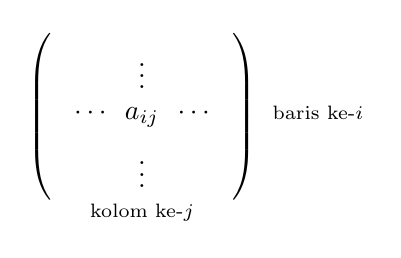
\begin{tikzpicture}[baseline]
			\matrix (M) [matrix of math nodes, left delimiter=(, right delimiter=)] {
				& \vdots & \\
				\cdots & a_{ij} & \cdots \\
				& \vdots & \\
			};
		\node[right=2.5em] at (M-2-3) {\scriptsize baris ke-$i$};
		\node[below=1em] at (M-3-2) {\scriptsize kolom ke-$j$};
	\end{tikzpicture}\]
	dan determinannya ditulis $\det A$. Perkalian matriks $AB=C$ ditentukan oleh $\sum_j a_{ij} b_{jk} = c_{ik}$. Transpos matriks $A$ ditulis ${}^t A$. Matriks identitas $n \times n$ ditulis $1_{n \times n}$ atau $1$.
\end{itemize}

\section*{Struktur aljabar yang umum}
Karena buku ini menitikberatkan interaksi antarkonsep, rujukan silang berskala kecil—atau dengan kata lain ``mendahului pembahasan''—tidak dapat dihindari selama hal itu tidak memengaruhi batang utama teori, terutama pada beberapa bab pertama. Banyaknya manfaat yang diperoleh pembaca bergantung pada pengetahuan yang telah dimiliki. Tabel berikut mencantumkan sejumlah struktur aljabar dasar, baik untuk memudahkan rujukan maupun untuk membantu pembaca menangkap atau mengingat kembali konsep-konsep awal aljabar dengan cepat.

Berikut ini $\GL_n(\R)$ menyatakan himpunan matriks real invertibel berukuran $n \times n$, $M_n(\R)$ menyatakan himpunan matriks real berukuran $n \times n$, dan $\Z/p\Z$ menyatakan sistem kelas residu modulo bilangan prima $p$.
\begin{center}
\scriptsize
\renewcommand{\arraystretch}{1.18}
\begin{tabularx}{\textwidth}{|>{\hsize=.65\hsize}Y|>{\hsize=1.10\hsize}Y|>{\hsize=1.35\hsize}Y|>{\hsize=1.15\hsize}Y|>{\hsize=.75\hsize}Y|} \hline
	\emph{Struktur} & \emph{Operasi} & \emph{Sifat} & \emph{Sifat homomorfisme $\phi$} & \emph{Contoh dasar} \\ \hline
	Himpunan $X$ & Tidak ada & Tidak ada & Pemetaan $X \xrightarrow{\phi} Y$ & $\{1,2,3, \ldots\}$ \\ \hline
	Monoid $M$ & Perkalian $(x,y) \mapsto xy$\newline Unsur identitas $1 \in M$ & Asosiativitas $x(yz)=(xy)z$\newline Sifat identitas $1x = x = x1$ & Pemetaan $M_1 \xrightarrow{\phi} M_2$\newline $\phi(xy)=\phi(x)\phi(y)$\newline $\phi(1)=1$ & $(\Z_{\geq 0}, +)$ \\ \hline
	Grup $G$ & Seperti di atas & Seperti di atas, dan $\forall x$ memiliki invers:\newline $xx^{-1} = 1 = x^{-1} x$ & Seperti di atas & $(\Z, +)$\newline $(\GL_n(\R), \cdot)$ \\ \hline
	Gelanggang $R$ & Grup abelian terhadap penjumlahan\newline Identitas penjumlahan $= 0$\newline Monoid terhadap perkalian\newline Identitas perkalian $= 1$ & Distributivitas:\newline $r(s+s') = rs+rs'$\newline $(s+s')r = sr + s'r$ & Homomorfisme terhadap penjumlahan dan perkalian & $(\Z, +, \cdot)$\newline Gelanggang polinom real\newline ($M_n(\R)$, $+$, $\cdot$) \\ \hline
	Medan $F$ & Seperti di atas & Seperti di atas, dan $\forall x \neq 0$ memiliki invers perkalian:\newline $xx^{-1}=1=x^{-1}x$\newline Perkalian komutatif $xy=yx$ & Seperti di atas & $\Q, \R, \CC$\newline $\Z/p\Z$ \\ \hline
	Modul kiri atas $R$: $M$ & Grup abelian terhadap penjumlahan\newline Perkalian skalar $R \times M \to M$ & $r(m + m') = rm + rm'$\newline $(r+r')m = rm + r'm$\newline $r(r'm) = (rr')m$\newline Sifat identitas $1 m = m$ & Homomorfisme terhadap penjumlahan\newline $\phi(rm) = r\phi(m)$ & Ruang vektor di atas suatu medan \\ \hline
\end{tabularx}
\end{center}

Sebagian pustaka tidak mensyaratkan keberadaan identitas perkalian pada gelanggang. Untuk setiap struktur dalam tabel di atas, pemetaan yang disebut homomorfisme memiliki sifat-sifat berikut:
\begin{compactitem}
	\item pemetaan identitas $\identity_X$ merupakan homomorfisme dari $X$ ke dirinya sendiri (disebut endomorfisme),
	\item komposisi homomorfisme tetap merupakan homomorfisme,
	\item komposisi homomorfisme memenuhi asosiativitas $f \circ (g \circ h)=(f \circ g) \circ h$.
\end{compactitem}
Jika sepasang homomorfisme antarstruktur $\begin{tikzcd} X \arrow[yshift=0.5ex, r, "f"] & Y \arrow[yshift=-0.5ex, l, "g"]\end{tikzcd}$ memenuhi $f \circ g = \identity_Y$ dan $g \circ f = \identity_X$, keduanya disebut saling invers. Dalam hal ini, $f$ dan $g$ saling menentukan secara tunggal; kita tulis $g = f^{-1}$ dan $f = g^{-1}$. Homomorfisme yang invertibel disebut isomorfisme. Ingatlah satu asas dasar aljabar: isomorfisme menghubungkan struktur aljabar yang pada hakikatnya sama.

Jika untuk sementara rincian teori himpunan diabaikan, sifat-sifat di atas menunjukkan bahwa untuk setiap jenis struktur dalam tabel, seluruh anggotanya (``objek'') bersama homomorfisme di antaranya (``morfisme'') membentuk contoh awal suatu \emph{kategori}. Kategori grup, grup abelian, dan modul kiri $R$ biasanya masing-masing ditulis $\cate{Grp}$, $\cate{Ab}$, dan $R\dcate{Mod}$; demikian pula untuk yang lain. Untuk objek $X$, $Y$ dalam kategori-kategori ini, semua homomorfisme di antaranya membentuk himpunan $\Hom_{\cate{Grp}}(X,Y)$, $\Hom_{\cate{Ab}}(X,Y)$, dan seterusnya, yang kerap disingkat menjadi $\Hom(X, Y)$. Homomorfisme dari $X$ ke dirinya sendiri disebut endomorfisme; semuanya membentuk monoid terhadap komposisi morfisme, yang ditulis $\End(X)$. Endomorfisme yang invertibel disebut automorfisme; automorfisme-automorfisme tersebut membentuk grup yang ditulis $\Aut(X)$.

Semua operasi pada struktur dalam tabel dibangun di atas himpunan. Untuk struktur-struktur itu dapat dibuktikan bahwa isomorfisme persis merupakan homomorfisme bijektif. Namun, perlu diperhatikan bahwa:
\begin{compactitem}
	\item suatu kategori tidak harus terdiri atas struktur yang dibangun di atas himpunan;
	\item dalam kategori lain yang objeknya berupa struktur berbasis himpunan, homomorfisme bijektif pun belum tentu invertibel. Contoh tandingan bakunya adalah kategori $\cate{Top}$ (objek = ruang topologis Hausdorff, morfisme = pemetaan kontinu). Isomorfisme di dalamnya adalah homeomorfisme ruang topologis, tetapi pemetaan kontinu yang bijektif belum tentu merupakan homeomorfisme.
\end{compactitem}

Dalam mengkaji homomorfisme antarstruktur, kami sering memakai bahasa diagram komutatif: panah menggambarkan homomorfisme, sedangkan komutativitas berarti bahwa komposisi panah di dalam diagram memberikan hasil yang sama melalui setiap lintasan. Contoh dasarnya ialah
\[\begin{tikzcd}
	A \arrow[r, "f"] \arrow[d, "h"'] & B \arrow[ld, "g"] \\
	C &
\end{tikzcd} \; \text{komutatif} \iff g \circ f = h. \]

Tentu saja, kami juga akan mempertimbangkan diagram yang lebih rumit, misalnya
\[\begin{tikzcd}[scale=0.6]
	A \arrow[r] \arrow[rd] & B \arrow[r] \arrow[d] & C \arrow[d] \\
	& D \arrow[r] & E
\end{tikzcd}\]
dan sebagainya; makna komutativitas dapat diperluas dengan cara yang sama. Komutativitas sebuah diagram dapat diperiksa bagian demi bagian. Misalnya, komutativitas diagram di atas dapat direduksi menjadi pemeriksaan subdiagram \begin{tikzcd} \bullet \arrow[r] \arrow[rd] & \bullet \arrow[d] \\ & \bullet \end{tikzcd} dan \begin{tikzcd} \bullet \arrow[r] \arrow[d] & \bullet \arrow[d] \\ \bullet \arrow[r] & \bullet \end{tikzcd}. Prosedur ini sangat berguna bagi diagram yang lebih rumit, misalnya dalam situasi ``tiga dimensi''.

Karena diagram komutatif hanya melibatkan komposisi panah, diagram tersebut berlaku pula dalam kategori umum.


	\backmatter
	\printbibliography[heading=bibintoc, title={Daftar Pustaka}]

	{\footnotesize
	\indexprologue{Istilah disusun menurut bentuk bahasa Indonesia; padanan bahasa Inggris dicantumkan bila berguna untuk penelusuran lintas bahasa.}
	\printindex
	}
\end{document}
